\section{Convexity}
\label{convexity}
In the following section convexity of the objective function is examined. 
Due to the reformulation of the objective function and constraints, the MPC optimization problem becomes the following: 

\begin{align}
\underset{\bm{\hat{u}_{Hp}}}{min} \:  \Upsilon(\bm{\hat{u}}_{\bm{Hp}}) &= \underset{\bm{\hat{u}_{Hp}}}{min} \:  \frac{1}{\eta}\bigg( \frac{1}{2} \bm{\hat{u}}_{\bm{Hp}}^{T} \bm{R} \bm{\hat{u}}_{\bm{Hp}} + \bm{b} \bm{\hat{u}}_{\bm{Hp}} + c \bigg)\\
\label{eq:obj_final1}
%
s.t. \:\:\:\:\:	&\begin{bmatrix}
		\bm{I} 	\\
		-\bm{I} 	\\
		\bm{L_{y}}	\\
		-\bm{L_{y}}	\\
		\bm{\Gamma}	\\
		-\bm{\Gamma}
	\end{bmatrix}
	\begin{matrix}
			\bm{\hat{u}_{Hp}}
	\end{matrix}
	\geq 
	\begin{bmatrix}
			\bm{\hat{u}_{1}}	\\
			\bm{\hat{u}_{2}}	\\
			\bm{\hat{y}_{1}}	\\
			\bm{\hat{y}_{2}}	\\
			\bm{\Delta \hat{p}_{wt,1}}	\\
			\bm{\Delta \hat{p}_{wt,2}}	
	\end{bmatrix}
\end{align}
\todo{source maybe}

\textbf{Objective function}

As shown, the objective function and the constraints are all written up according to the small-signal value of the control signal. The difficulty of solving this optimization problem simplifies however, if $\Upsilon$ is convex. This is due to the fact that if the objective function is convex then any local minima are also the global minimum. 
\\
The function, $\Upsilon$, defines a quadratic surface. If this surface is convex, then it can be visualized as in \figref{convexfig}. If the objective function is non-convex, the surface has a form such as in \figref{nonconvexfig}. 

\begin{figure}[H]
  \centering
  \begin{minipage}[b]{0.45\textwidth}
    % This file was created by matlab2tikz.
%
%The latest updates can be retrieved from
%  http://www.mathworks.com/matlabcentral/fileexchange/22022-matlab2tikz-matlab2tikz
%where you can also make suggestions and rate matlab2tikz.
%
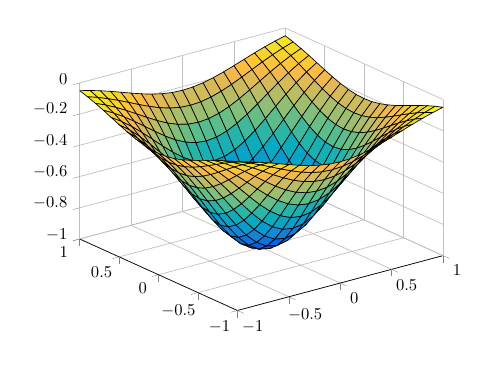
\begin{tikzpicture}[scale=0.6]

\begin{axis}[%
width=3.028in,
height=2.354in,
at={(0.011in,0.042in)},
scale only axis,
xmin=-1,
xmax=1,
tick align=outside,
xmajorgrids,
xtick = {-1,-0.5,0,0.5,1},
ymin=-1,
ymax=1,
ymajorgrids,
ytick = {-1,-0.5,0,0.5,1},
zmin=-1,
zmax=0,
zmajorgrids,
ztick = {-1,-0.8,-0.6,-0.4,-0.2,0},
view={-37.5}{30},
axis background/.style={fill=white},
axis x line*=bottom,
axis y line*=left,
axis z line*=left
]

\addplot3[%
surf,
shader=flat corner,draw=black,z buffer=sort,colormap={mymap}{[1pt] rgb(0pt)=(0.2081,0.1663,0.5292); rgb(1pt)=(0.211624,0.189781,0.577676); rgb(2pt)=(0.212252,0.213771,0.626971); rgb(3pt)=(0.2081,0.2386,0.677086); rgb(4pt)=(0.195905,0.264457,0.7279); rgb(5pt)=(0.170729,0.291938,0.779248); rgb(6pt)=(0.125271,0.324243,0.830271); rgb(7pt)=(0.0591333,0.359833,0.868333); rgb(8pt)=(0.0116952,0.38751,0.881957); rgb(9pt)=(0.00595714,0.408614,0.882843); rgb(10pt)=(0.0165143,0.4266,0.878633); rgb(11pt)=(0.0328524,0.443043,0.871957); rgb(12pt)=(0.0498143,0.458571,0.864057); rgb(13pt)=(0.0629333,0.47369,0.855438); rgb(14pt)=(0.0722667,0.488667,0.8467); rgb(15pt)=(0.0779429,0.503986,0.838371); rgb(16pt)=(0.0793476,0.520024,0.831181); rgb(17pt)=(0.0749429,0.537543,0.826271); rgb(18pt)=(0.0640571,0.556986,0.823957); rgb(19pt)=(0.0487714,0.577224,0.822829); rgb(20pt)=(0.0343429,0.596581,0.819852); rgb(21pt)=(0.0265,0.6137,0.8135); rgb(22pt)=(0.0238905,0.628662,0.803762); rgb(23pt)=(0.0230905,0.641786,0.791267); rgb(24pt)=(0.0227714,0.653486,0.776757); rgb(25pt)=(0.0266619,0.664195,0.760719); rgb(26pt)=(0.0383714,0.674271,0.743552); rgb(27pt)=(0.0589714,0.683757,0.725386); rgb(28pt)=(0.0843,0.692833,0.706167); rgb(29pt)=(0.113295,0.7015,0.685857); rgb(30pt)=(0.145271,0.709757,0.664629); rgb(31pt)=(0.180133,0.717657,0.642433); rgb(32pt)=(0.217829,0.725043,0.619262); rgb(33pt)=(0.258643,0.731714,0.595429); rgb(34pt)=(0.302171,0.737605,0.571186); rgb(35pt)=(0.348167,0.742433,0.547267); rgb(36pt)=(0.395257,0.7459,0.524443); rgb(37pt)=(0.44201,0.748081,0.503314); rgb(38pt)=(0.487124,0.749062,0.483976); rgb(39pt)=(0.530029,0.749114,0.466114); rgb(40pt)=(0.570857,0.748519,0.44939); rgb(41pt)=(0.609852,0.747314,0.433686); rgb(42pt)=(0.6473,0.7456,0.4188); rgb(43pt)=(0.683419,0.743476,0.404433); rgb(44pt)=(0.71841,0.741133,0.390476); rgb(45pt)=(0.752486,0.7384,0.376814); rgb(46pt)=(0.785843,0.735567,0.363271); rgb(47pt)=(0.818505,0.732733,0.34979); rgb(48pt)=(0.850657,0.7299,0.336029); rgb(49pt)=(0.882433,0.727433,0.3217); rgb(50pt)=(0.913933,0.725786,0.306276); rgb(51pt)=(0.944957,0.726114,0.288643); rgb(52pt)=(0.973895,0.731395,0.266648); rgb(53pt)=(0.993771,0.745457,0.240348); rgb(54pt)=(0.999043,0.765314,0.216414); rgb(55pt)=(0.995533,0.786057,0.196652); rgb(56pt)=(0.988,0.8066,0.179367); rgb(57pt)=(0.978857,0.827143,0.163314); rgb(58pt)=(0.9697,0.848138,0.147452); rgb(59pt)=(0.962586,0.870514,0.1309); rgb(60pt)=(0.958871,0.8949,0.113243); rgb(61pt)=(0.959824,0.921833,0.0948381); rgb(62pt)=(0.9661,0.951443,0.0755333); rgb(63pt)=(0.9763,0.9831,0.0538)},mesh/rows=21]
table[row sep=crcr, point meta=\thisrow{c}] {%
%
x	y	z	c\\
-1	-1	-0.0497870683678639	-0.0497870683678639\\
-1	-0.9	-0.0662049530070732	-0.0662049530070732\\
-1	-0.8	-0.0854349509673212	-0.0854349509673212\\
-1	-0.7	-0.106992129853114	-0.106992129853114\\
-1	-0.6	-0.130028710878426	-0.130028710878426\\
-1	-0.5	-0.153354966844928	-0.153354966844928\\
-1	-0.4	-0.175520400616997	-0.175520400616997\\
-1	-0.3	-0.194952371299182	-0.194952371299182\\
-1	-0.2	-0.210136071200765	-0.210136071200765\\
-1	-0.1	-0.219808184847762	-0.219808184847762\\
-1	0	-0.22313016014843	-0.22313016014843\\
-1	0.1	-0.219808184847762	-0.219808184847762\\
-1	0.2	-0.210136071200765	-0.210136071200765\\
-1	0.3	-0.194952371299182	-0.194952371299182\\
-1	0.4	-0.175520400616997	-0.175520400616997\\
-1	0.5	-0.153354966844928	-0.153354966844928\\
-1	0.6	-0.130028710878426	-0.130028710878426\\
-1	0.7	-0.106992129853114	-0.106992129853114\\
-1	0.8	-0.0854349509673212	-0.0854349509673212\\
-1	0.9	-0.0662049530070732	-0.0662049530070732\\
-1	1	-0.0497870683678639	-0.0497870683678639\\
-0.9	-1	-0.0662049530070732	-0.0662049530070732\\
-0.9	-0.9	-0.0880368325823725	-0.0880368325823725\\
-0.9	-0.8	-0.113608153670764	-0.113608153670764\\
-0.9	-0.7	-0.142274071586514	-0.142274071586514\\
-0.9	-0.6	-0.172907242291716	-0.172907242291716\\
-0.9	-0.5	-0.203925611734213	-0.203925611734213\\
-0.9	-0.4	-0.233400363901151	-0.233400363901151\\
-0.9	-0.3	-0.259240260645892	-0.259240260645892\\
-0.9	-0.2	-0.279430968221407	-0.279430968221407\\
-0.9	-0.1	-0.292292577680859	-0.292292577680859\\
-0.9	0	-0.296710014294045	-0.296710014294045\\
-0.9	0.1	-0.292292577680859	-0.292292577680859\\
-0.9	0.2	-0.279430968221407	-0.279430968221407\\
-0.9	0.3	-0.259240260645892	-0.259240260645892\\
-0.9	0.4	-0.233400363901151	-0.233400363901151\\
-0.9	0.5	-0.203925611734213	-0.203925611734213\\
-0.9	0.6	-0.172907242291716	-0.172907242291716\\
-0.9	0.7	-0.142274071586514	-0.142274071586514\\
-0.9	0.8	-0.113608153670764	-0.113608153670764\\
-0.9	0.9	-0.0880368325823725	-0.0880368325823725\\
-0.9	1	-0.0662049530070732	-0.0662049530070732\\
-0.8	-1	-0.0854349509673212	-0.0854349509673212\\
-0.8	-0.9	-0.113608153670764	-0.113608153670764\\
-0.8	-0.8	-0.14660696213035	-0.14660696213035\\
-0.8	-0.7	-0.183599229027718	-0.183599229027718\\
-0.8	-0.6	-0.22313016014843	-0.22313016014843\\
-0.8	-0.5	-0.263158175456029	-0.263158175456029\\
-0.8	-0.4	-0.301194211912202	-0.301194211912202\\
-0.8	-0.3	-0.334539606948608	-0.334539606948608\\
-0.8	-0.2	-0.360594940173078	-0.360594940173078\\
-0.8	-0.1	-0.377192353563157	-0.377192353563157\\
-0.8	0	-0.382892885975112	-0.382892885975112\\
-0.8	0.1	-0.377192353563157	-0.377192353563157\\
-0.8	0.2	-0.360594940173078	-0.360594940173078\\
-0.8	0.3	-0.334539606948608	-0.334539606948608\\
-0.8	0.4	-0.301194211912202	-0.301194211912202\\
-0.8	0.5	-0.263158175456029	-0.263158175456029\\
-0.8	0.6	-0.22313016014843	-0.22313016014843\\
-0.8	0.7	-0.183599229027718	-0.183599229027718\\
-0.8	0.8	-0.14660696213035	-0.14660696213035\\
-0.8	0.9	-0.113608153670764	-0.113608153670764\\
-0.8	1	-0.0854349509673212	-0.0854349509673212\\
-0.7	-1	-0.106992129853114	-0.106992129853114\\
-0.7	-0.9	-0.142274071586514	-0.142274071586514\\
-0.7	-0.8	-0.183599229027718	-0.183599229027718\\
-0.7	-0.7	-0.229925485186724	-0.229925485186724\\
-0.7	-0.6	-0.279430968221407	-0.279430968221407\\
-0.7	-0.5	-0.329558961075189	-0.329558961075189\\
-0.7	-0.4	-0.377192353563157	-0.377192353563157\\
-0.7	-0.3	-0.418951549247639	-0.418951549247639\\
-0.7	-0.2	-0.451581234922592	-0.451581234922592\\
-0.7	-0.1	-0.472366552741015	-0.472366552741015\\
-0.7	0	-0.479505458974894	-0.479505458974894\\
-0.7	0.1	-0.472366552741015	-0.472366552741015\\
-0.7	0.2	-0.451581234922592	-0.451581234922592\\
-0.7	0.3	-0.418951549247639	-0.418951549247639\\
-0.7	0.4	-0.377192353563157	-0.377192353563157\\
-0.7	0.5	-0.329558961075189	-0.329558961075189\\
-0.7	0.6	-0.279430968221407	-0.279430968221407\\
-0.7	0.7	-0.229925485186724	-0.229925485186724\\
-0.7	0.8	-0.183599229027718	-0.183599229027718\\
-0.7	0.9	-0.142274071586514	-0.142274071586514\\
-0.7	1	-0.106992129853114	-0.106992129853114\\
-0.6	-1	-0.130028710878426	-0.130028710878426\\
-0.6	-0.9	-0.172907242291716	-0.172907242291716\\
-0.6	-0.8	-0.22313016014843	-0.22313016014843\\
-0.6	-0.7	-0.279430968221407	-0.279430968221407\\
-0.6	-0.6	-0.339595525644939	-0.339595525644939\\
-0.6	-0.5	-0.400516626090819	-0.400516626090819\\
-0.6	-0.4	-0.458406011305224	-0.458406011305224\\
-0.6	-0.3	-0.509156420607549	-0.509156420607549\\
-0.6	-0.2	-0.548811636094027	-0.548811636094027\\
-0.6	-0.1	-0.574072261196436	-0.574072261196436\\
-0.6	0	-0.58274825237399	-0.58274825237399\\
-0.6	0.1	-0.574072261196436	-0.574072261196436\\
-0.6	0.2	-0.548811636094027	-0.548811636094027\\
-0.6	0.3	-0.509156420607549	-0.509156420607549\\
-0.6	0.4	-0.458406011305224	-0.458406011305224\\
-0.6	0.5	-0.400516626090819	-0.400516626090819\\
-0.6	0.6	-0.339595525644939	-0.339595525644939\\
-0.6	0.7	-0.279430968221407	-0.279430968221407\\
-0.6	0.8	-0.22313016014843	-0.22313016014843\\
-0.6	0.9	-0.172907242291716	-0.172907242291716\\
-0.6	1	-0.130028710878426	-0.130028710878426\\
-0.5	-1	-0.153354966844928	-0.153354966844928\\
-0.5	-0.9	-0.203925611734213	-0.203925611734213\\
-0.5	-0.8	-0.263158175456029	-0.263158175456029\\
-0.5	-0.7	-0.329558961075189	-0.329558961075189\\
-0.5	-0.6	-0.400516626090819	-0.400516626090819\\
-0.5	-0.5	-0.472366552741015	-0.472366552741015\\
-0.5	-0.4	-0.540640895309317	-0.540640895309317\\
-0.5	-0.3	-0.600495578812266	-0.600495578812266\\
-0.5	-0.2	-0.647264667078035	-0.647264667078035\\
-0.5	-0.1	-0.677056874498165	-0.677056874498165\\
-0.5	0	-0.687289278790972	-0.687289278790972\\
-0.5	0.1	-0.677056874498165	-0.677056874498165\\
-0.5	0.2	-0.647264667078035	-0.647264667078035\\
-0.5	0.3	-0.600495578812266	-0.600495578812266\\
-0.5	0.4	-0.540640895309317	-0.540640895309317\\
-0.5	0.5	-0.472366552741015	-0.472366552741015\\
-0.5	0.6	-0.400516626090819	-0.400516626090819\\
-0.5	0.7	-0.329558961075189	-0.329558961075189\\
-0.5	0.8	-0.263158175456029	-0.263158175456029\\
-0.5	0.9	-0.203925611734213	-0.203925611734213\\
-0.5	1	-0.153354966844928	-0.153354966844928\\
-0.4	-1	-0.175520400616997	-0.175520400616997\\
-0.4	-0.9	-0.233400363901151	-0.233400363901151\\
-0.4	-0.8	-0.301194211912202	-0.301194211912202\\
-0.4	-0.7	-0.377192353563157	-0.377192353563157\\
-0.4	-0.6	-0.458406011305224	-0.458406011305224\\
-0.4	-0.5	-0.540640895309317	-0.540640895309317\\
-0.4	-0.4	-0.618783391806141	-0.618783391806141\\
-0.4	-0.3	-0.687289278790972	-0.687289278790972\\
-0.4	-0.2	-0.740818220681718	-0.740818220681718\\
-0.4	-0.1	-0.774916497961081	-0.774916497961081\\
-0.4	0	-0.786627861066553	-0.786627861066553\\
-0.4	0.1	-0.774916497961081	-0.774916497961081\\
-0.4	0.2	-0.740818220681718	-0.740818220681718\\
-0.4	0.3	-0.687289278790972	-0.687289278790972\\
-0.4	0.4	-0.618783391806141	-0.618783391806141\\
-0.4	0.5	-0.540640895309317	-0.540640895309317\\
-0.4	0.6	-0.458406011305224	-0.458406011305224\\
-0.4	0.7	-0.377192353563157	-0.377192353563157\\
-0.4	0.8	-0.301194211912202	-0.301194211912202\\
-0.4	0.9	-0.233400363901151	-0.233400363901151\\
-0.4	1	-0.175520400616997	-0.175520400616997\\
-0.3	-1	-0.194952371299182	-0.194952371299182\\
-0.3	-0.9	-0.259240260645892	-0.259240260645892\\
-0.3	-0.8	-0.334539606948608	-0.334539606948608\\
-0.3	-0.7	-0.418951549247639	-0.418951549247639\\
-0.3	-0.6	-0.509156420607549	-0.509156420607549\\
-0.3	-0.5	-0.600495578812266	-0.600495578812266\\
-0.3	-0.4	-0.687289278790972	-0.687289278790972\\
-0.3	-0.3	-0.763379494336853	-0.763379494336853\\
-0.3	-0.2	-0.822834658056018	-0.822834658056018\\
-0.3	-0.1	-0.860707976425058	-0.860707976425058\\
-0.3	0	-0.873715911688035	-0.873715911688035\\
-0.3	0.1	-0.860707976425058	-0.860707976425058\\
-0.3	0.2	-0.822834658056018	-0.822834658056018\\
-0.3	0.3	-0.763379494336853	-0.763379494336853\\
-0.3	0.4	-0.687289278790972	-0.687289278790972\\
-0.3	0.5	-0.600495578812266	-0.600495578812266\\
-0.3	0.6	-0.509156420607549	-0.509156420607549\\
-0.3	0.7	-0.418951549247639	-0.418951549247639\\
-0.3	0.8	-0.334539606948608	-0.334539606948608\\
-0.3	0.9	-0.259240260645892	-0.259240260645892\\
-0.3	1	-0.194952371299182	-0.194952371299182\\
-0.2	-1	-0.210136071200765	-0.210136071200765\\
-0.2	-0.9	-0.279430968221407	-0.279430968221407\\
-0.2	-0.8	-0.360594940173078	-0.360594940173078\\
-0.2	-0.7	-0.451581234922592	-0.451581234922592\\
-0.2	-0.6	-0.548811636094027	-0.548811636094027\\
-0.2	-0.5	-0.647264667078035	-0.647264667078035\\
-0.2	-0.4	-0.740818220681718	-0.740818220681718\\
-0.2	-0.3	-0.822834658056018	-0.822834658056018\\
-0.2	-0.2	-0.886920436717158	-0.886920436717158\\
-0.2	-0.1	-0.927743486328553	-0.927743486328553\\
-0.2	0	-0.941764533584249	-0.941764533584249\\
-0.2	0.1	-0.927743486328553	-0.927743486328553\\
-0.2	0.2	-0.886920436717158	-0.886920436717158\\
-0.2	0.3	-0.822834658056018	-0.822834658056018\\
-0.2	0.4	-0.740818220681718	-0.740818220681718\\
-0.2	0.5	-0.647264667078035	-0.647264667078035\\
-0.2	0.6	-0.548811636094027	-0.548811636094027\\
-0.2	0.7	-0.451581234922592	-0.451581234922592\\
-0.2	0.8	-0.360594940173078	-0.360594940173078\\
-0.2	0.9	-0.279430968221407	-0.279430968221407\\
-0.2	1	-0.210136071200765	-0.210136071200765\\
-0.1	-1	-0.219808184847762	-0.219808184847762\\
-0.1	-0.9	-0.292292577680859	-0.292292577680859\\
-0.1	-0.8	-0.377192353563157	-0.377192353563157\\
-0.1	-0.7	-0.472366552741015	-0.472366552741015\\
-0.1	-0.6	-0.574072261196436	-0.574072261196436\\
-0.1	-0.5	-0.677056874498165	-0.677056874498165\\
-0.1	-0.4	-0.774916497961081	-0.774916497961081\\
-0.1	-0.3	-0.860707976425058	-0.860707976425058\\
-0.1	-0.2	-0.927743486328553	-0.927743486328553\\
-0.1	-0.1	-0.970445533548508	-0.970445533548508\\
-0.1	0	-0.985111939603063	-0.985111939603063\\
-0.1	0.1	-0.970445533548508	-0.970445533548508\\
-0.1	0.2	-0.927743486328553	-0.927743486328553\\
-0.1	0.3	-0.860707976425058	-0.860707976425058\\
-0.1	0.4	-0.774916497961081	-0.774916497961081\\
-0.1	0.5	-0.677056874498165	-0.677056874498165\\
-0.1	0.6	-0.574072261196436	-0.574072261196436\\
-0.1	0.7	-0.472366552741015	-0.472366552741015\\
-0.1	0.8	-0.377192353563157	-0.377192353563157\\
-0.1	0.9	-0.292292577680859	-0.292292577680859\\
-0.1	1	-0.219808184847762	-0.219808184847762\\
0	-1	-0.22313016014843	-0.22313016014843\\
0	-0.9	-0.296710014294045	-0.296710014294045\\
0	-0.8	-0.382892885975112	-0.382892885975112\\
0	-0.7	-0.479505458974894	-0.479505458974894\\
0	-0.6	-0.58274825237399	-0.58274825237399\\
0	-0.5	-0.687289278790972	-0.687289278790972\\
0	-0.4	-0.786627861066553	-0.786627861066553\\
0	-0.3	-0.873715911688035	-0.873715911688035\\
0	-0.2	-0.941764533584249	-0.941764533584249\\
0	-0.1	-0.985111939603063	-0.985111939603063\\
0	0	-1	-1\\
0	0.1	-0.985111939603063	-0.985111939603063\\
0	0.2	-0.941764533584249	-0.941764533584249\\
0	0.3	-0.873715911688035	-0.873715911688035\\
0	0.4	-0.786627861066553	-0.786627861066553\\
0	0.5	-0.687289278790972	-0.687289278790972\\
0	0.6	-0.58274825237399	-0.58274825237399\\
0	0.7	-0.479505458974894	-0.479505458974894\\
0	0.8	-0.382892885975112	-0.382892885975112\\
0	0.9	-0.296710014294045	-0.296710014294045\\
0	1	-0.22313016014843	-0.22313016014843\\
0.1	-1	-0.219808184847762	-0.219808184847762\\
0.1	-0.9	-0.292292577680859	-0.292292577680859\\
0.1	-0.8	-0.377192353563157	-0.377192353563157\\
0.1	-0.7	-0.472366552741015	-0.472366552741015\\
0.1	-0.6	-0.574072261196436	-0.574072261196436\\
0.1	-0.5	-0.677056874498165	-0.677056874498165\\
0.1	-0.4	-0.774916497961081	-0.774916497961081\\
0.1	-0.3	-0.860707976425058	-0.860707976425058\\
0.1	-0.2	-0.927743486328553	-0.927743486328553\\
0.1	-0.1	-0.970445533548508	-0.970445533548508\\
0.1	0	-0.985111939603063	-0.985111939603063\\
0.1	0.1	-0.970445533548508	-0.970445533548508\\
0.1	0.2	-0.927743486328553	-0.927743486328553\\
0.1	0.3	-0.860707976425058	-0.860707976425058\\
0.1	0.4	-0.774916497961081	-0.774916497961081\\
0.1	0.5	-0.677056874498165	-0.677056874498165\\
0.1	0.6	-0.574072261196436	-0.574072261196436\\
0.1	0.7	-0.472366552741015	-0.472366552741015\\
0.1	0.8	-0.377192353563157	-0.377192353563157\\
0.1	0.9	-0.292292577680859	-0.292292577680859\\
0.1	1	-0.219808184847762	-0.219808184847762\\
0.2	-1	-0.210136071200765	-0.210136071200765\\
0.2	-0.9	-0.279430968221407	-0.279430968221407\\
0.2	-0.8	-0.360594940173078	-0.360594940173078\\
0.2	-0.7	-0.451581234922592	-0.451581234922592\\
0.2	-0.6	-0.548811636094027	-0.548811636094027\\
0.2	-0.5	-0.647264667078035	-0.647264667078035\\
0.2	-0.4	-0.740818220681718	-0.740818220681718\\
0.2	-0.3	-0.822834658056018	-0.822834658056018\\
0.2	-0.2	-0.886920436717158	-0.886920436717158\\
0.2	-0.1	-0.927743486328553	-0.927743486328553\\
0.2	0	-0.941764533584249	-0.941764533584249\\
0.2	0.1	-0.927743486328553	-0.927743486328553\\
0.2	0.2	-0.886920436717158	-0.886920436717158\\
0.2	0.3	-0.822834658056018	-0.822834658056018\\
0.2	0.4	-0.740818220681718	-0.740818220681718\\
0.2	0.5	-0.647264667078035	-0.647264667078035\\
0.2	0.6	-0.548811636094027	-0.548811636094027\\
0.2	0.7	-0.451581234922592	-0.451581234922592\\
0.2	0.8	-0.360594940173078	-0.360594940173078\\
0.2	0.9	-0.279430968221407	-0.279430968221407\\
0.2	1	-0.210136071200765	-0.210136071200765\\
0.3	-1	-0.194952371299182	-0.194952371299182\\
0.3	-0.9	-0.259240260645892	-0.259240260645892\\
0.3	-0.8	-0.334539606948608	-0.334539606948608\\
0.3	-0.7	-0.418951549247639	-0.418951549247639\\
0.3	-0.6	-0.509156420607549	-0.509156420607549\\
0.3	-0.5	-0.600495578812266	-0.600495578812266\\
0.3	-0.4	-0.687289278790972	-0.687289278790972\\
0.3	-0.3	-0.763379494336853	-0.763379494336853\\
0.3	-0.2	-0.822834658056018	-0.822834658056018\\
0.3	-0.1	-0.860707976425058	-0.860707976425058\\
0.3	0	-0.873715911688035	-0.873715911688035\\
0.3	0.1	-0.860707976425058	-0.860707976425058\\
0.3	0.2	-0.822834658056018	-0.822834658056018\\
0.3	0.3	-0.763379494336853	-0.763379494336853\\
0.3	0.4	-0.687289278790972	-0.687289278790972\\
0.3	0.5	-0.600495578812266	-0.600495578812266\\
0.3	0.6	-0.509156420607549	-0.509156420607549\\
0.3	0.7	-0.418951549247639	-0.418951549247639\\
0.3	0.8	-0.334539606948608	-0.334539606948608\\
0.3	0.9	-0.259240260645892	-0.259240260645892\\
0.3	1	-0.194952371299182	-0.194952371299182\\
0.4	-1	-0.175520400616997	-0.175520400616997\\
0.4	-0.9	-0.233400363901151	-0.233400363901151\\
0.4	-0.8	-0.301194211912202	-0.301194211912202\\
0.4	-0.7	-0.377192353563157	-0.377192353563157\\
0.4	-0.6	-0.458406011305224	-0.458406011305224\\
0.4	-0.5	-0.540640895309317	-0.540640895309317\\
0.4	-0.4	-0.618783391806141	-0.618783391806141\\
0.4	-0.3	-0.687289278790972	-0.687289278790972\\
0.4	-0.2	-0.740818220681718	-0.740818220681718\\
0.4	-0.1	-0.774916497961081	-0.774916497961081\\
0.4	0	-0.786627861066553	-0.786627861066553\\
0.4	0.1	-0.774916497961081	-0.774916497961081\\
0.4	0.2	-0.740818220681718	-0.740818220681718\\
0.4	0.3	-0.687289278790972	-0.687289278790972\\
0.4	0.4	-0.618783391806141	-0.618783391806141\\
0.4	0.5	-0.540640895309317	-0.540640895309317\\
0.4	0.6	-0.458406011305224	-0.458406011305224\\
0.4	0.7	-0.377192353563157	-0.377192353563157\\
0.4	0.8	-0.301194211912202	-0.301194211912202\\
0.4	0.9	-0.233400363901151	-0.233400363901151\\
0.4	1	-0.175520400616997	-0.175520400616997\\
0.5	-1	-0.153354966844928	-0.153354966844928\\
0.5	-0.9	-0.203925611734213	-0.203925611734213\\
0.5	-0.8	-0.263158175456029	-0.263158175456029\\
0.5	-0.7	-0.329558961075189	-0.329558961075189\\
0.5	-0.6	-0.400516626090819	-0.400516626090819\\
0.5	-0.5	-0.472366552741015	-0.472366552741015\\
0.5	-0.4	-0.540640895309317	-0.540640895309317\\
0.5	-0.3	-0.600495578812266	-0.600495578812266\\
0.5	-0.2	-0.647264667078035	-0.647264667078035\\
0.5	-0.1	-0.677056874498165	-0.677056874498165\\
0.5	0	-0.687289278790972	-0.687289278790972\\
0.5	0.1	-0.677056874498165	-0.677056874498165\\
0.5	0.2	-0.647264667078035	-0.647264667078035\\
0.5	0.3	-0.600495578812266	-0.600495578812266\\
0.5	0.4	-0.540640895309317	-0.540640895309317\\
0.5	0.5	-0.472366552741015	-0.472366552741015\\
0.5	0.6	-0.400516626090819	-0.400516626090819\\
0.5	0.7	-0.329558961075189	-0.329558961075189\\
0.5	0.8	-0.263158175456029	-0.263158175456029\\
0.5	0.9	-0.203925611734213	-0.203925611734213\\
0.5	1	-0.153354966844928	-0.153354966844928\\
0.6	-1	-0.130028710878426	-0.130028710878426\\
0.6	-0.9	-0.172907242291716	-0.172907242291716\\
0.6	-0.8	-0.22313016014843	-0.22313016014843\\
0.6	-0.7	-0.279430968221407	-0.279430968221407\\
0.6	-0.6	-0.339595525644939	-0.339595525644939\\
0.6	-0.5	-0.400516626090819	-0.400516626090819\\
0.6	-0.4	-0.458406011305224	-0.458406011305224\\
0.6	-0.3	-0.509156420607549	-0.509156420607549\\
0.6	-0.2	-0.548811636094027	-0.548811636094027\\
0.6	-0.1	-0.574072261196436	-0.574072261196436\\
0.6	0	-0.58274825237399	-0.58274825237399\\
0.6	0.1	-0.574072261196436	-0.574072261196436\\
0.6	0.2	-0.548811636094027	-0.548811636094027\\
0.6	0.3	-0.509156420607549	-0.509156420607549\\
0.6	0.4	-0.458406011305224	-0.458406011305224\\
0.6	0.5	-0.400516626090819	-0.400516626090819\\
0.6	0.6	-0.339595525644939	-0.339595525644939\\
0.6	0.7	-0.279430968221407	-0.279430968221407\\
0.6	0.8	-0.22313016014843	-0.22313016014843\\
0.6	0.9	-0.172907242291716	-0.172907242291716\\
0.6	1	-0.130028710878426	-0.130028710878426\\
0.7	-1	-0.106992129853114	-0.106992129853114\\
0.7	-0.9	-0.142274071586514	-0.142274071586514\\
0.7	-0.8	-0.183599229027718	-0.183599229027718\\
0.7	-0.7	-0.229925485186724	-0.229925485186724\\
0.7	-0.6	-0.279430968221407	-0.279430968221407\\
0.7	-0.5	-0.329558961075189	-0.329558961075189\\
0.7	-0.4	-0.377192353563157	-0.377192353563157\\
0.7	-0.3	-0.418951549247639	-0.418951549247639\\
0.7	-0.2	-0.451581234922592	-0.451581234922592\\
0.7	-0.1	-0.472366552741015	-0.472366552741015\\
0.7	0	-0.479505458974894	-0.479505458974894\\
0.7	0.1	-0.472366552741015	-0.472366552741015\\
0.7	0.2	-0.451581234922592	-0.451581234922592\\
0.7	0.3	-0.418951549247639	-0.418951549247639\\
0.7	0.4	-0.377192353563157	-0.377192353563157\\
0.7	0.5	-0.329558961075189	-0.329558961075189\\
0.7	0.6	-0.279430968221407	-0.279430968221407\\
0.7	0.7	-0.229925485186724	-0.229925485186724\\
0.7	0.8	-0.183599229027718	-0.183599229027718\\
0.7	0.9	-0.142274071586514	-0.142274071586514\\
0.7	1	-0.106992129853114	-0.106992129853114\\
0.8	-1	-0.0854349509673212	-0.0854349509673212\\
0.8	-0.9	-0.113608153670764	-0.113608153670764\\
0.8	-0.8	-0.14660696213035	-0.14660696213035\\
0.8	-0.7	-0.183599229027718	-0.183599229027718\\
0.8	-0.6	-0.22313016014843	-0.22313016014843\\
0.8	-0.5	-0.263158175456029	-0.263158175456029\\
0.8	-0.4	-0.301194211912202	-0.301194211912202\\
0.8	-0.3	-0.334539606948608	-0.334539606948608\\
0.8	-0.2	-0.360594940173078	-0.360594940173078\\
0.8	-0.1	-0.377192353563157	-0.377192353563157\\
0.8	0	-0.382892885975112	-0.382892885975112\\
0.8	0.1	-0.377192353563157	-0.377192353563157\\
0.8	0.2	-0.360594940173078	-0.360594940173078\\
0.8	0.3	-0.334539606948608	-0.334539606948608\\
0.8	0.4	-0.301194211912202	-0.301194211912202\\
0.8	0.5	-0.263158175456029	-0.263158175456029\\
0.8	0.6	-0.22313016014843	-0.22313016014843\\
0.8	0.7	-0.183599229027718	-0.183599229027718\\
0.8	0.8	-0.14660696213035	-0.14660696213035\\
0.8	0.9	-0.113608153670764	-0.113608153670764\\
0.8	1	-0.0854349509673212	-0.0854349509673212\\
0.9	-1	-0.0662049530070732	-0.0662049530070732\\
0.9	-0.9	-0.0880368325823725	-0.0880368325823725\\
0.9	-0.8	-0.113608153670764	-0.113608153670764\\
0.9	-0.7	-0.142274071586514	-0.142274071586514\\
0.9	-0.6	-0.172907242291716	-0.172907242291716\\
0.9	-0.5	-0.203925611734213	-0.203925611734213\\
0.9	-0.4	-0.233400363901151	-0.233400363901151\\
0.9	-0.3	-0.259240260645892	-0.259240260645892\\
0.9	-0.2	-0.279430968221407	-0.279430968221407\\
0.9	-0.1	-0.292292577680859	-0.292292577680859\\
0.9	0	-0.296710014294045	-0.296710014294045\\
0.9	0.1	-0.292292577680859	-0.292292577680859\\
0.9	0.2	-0.279430968221407	-0.279430968221407\\
0.9	0.3	-0.259240260645892	-0.259240260645892\\
0.9	0.4	-0.233400363901151	-0.233400363901151\\
0.9	0.5	-0.203925611734213	-0.203925611734213\\
0.9	0.6	-0.172907242291716	-0.172907242291716\\
0.9	0.7	-0.142274071586514	-0.142274071586514\\
0.9	0.8	-0.113608153670764	-0.113608153670764\\
0.9	0.9	-0.0880368325823725	-0.0880368325823725\\
0.9	1	-0.0662049530070732	-0.0662049530070732\\
1	-1	-0.0497870683678639	-0.0497870683678639\\
1	-0.9	-0.0662049530070732	-0.0662049530070732\\
1	-0.8	-0.0854349509673212	-0.0854349509673212\\
1	-0.7	-0.106992129853114	-0.106992129853114\\
1	-0.6	-0.130028710878426	-0.130028710878426\\
1	-0.5	-0.153354966844928	-0.153354966844928\\
1	-0.4	-0.175520400616997	-0.175520400616997\\
1	-0.3	-0.194952371299182	-0.194952371299182\\
1	-0.2	-0.210136071200765	-0.210136071200765\\
1	-0.1	-0.219808184847762	-0.219808184847762\\
1	0	-0.22313016014843	-0.22313016014843\\
1	0.1	-0.219808184847762	-0.219808184847762\\
1	0.2	-0.210136071200765	-0.210136071200765\\
1	0.3	-0.194952371299182	-0.194952371299182\\
1	0.4	-0.175520400616997	-0.175520400616997\\
1	0.5	-0.153354966844928	-0.153354966844928\\
1	0.6	-0.130028710878426	-0.130028710878426\\
1	0.7	-0.106992129853114	-0.106992129853114\\
1	0.8	-0.0854349509673212	-0.0854349509673212\\
1	0.9	-0.0662049530070732	-0.0662049530070732\\
1	1	-0.0497870683678639	-0.0497870683678639\\
};
\end{axis}
\end{tikzpicture}% 
    \caption{Quadratic convex surface.}
    \label{convexfig}
  \end{minipage}
  \hfill
  \begin{minipage}[b]{0.45\textwidth}
    % This file was created by matlab2tikz.
%
%The latest updates can be retrieved from
%  http://www.mathworks.com/matlabcentral/fileexchange/22022-matlab2tikz-matlab2tikz
%where you can also make suggestions and rate matlab2tikz.
%
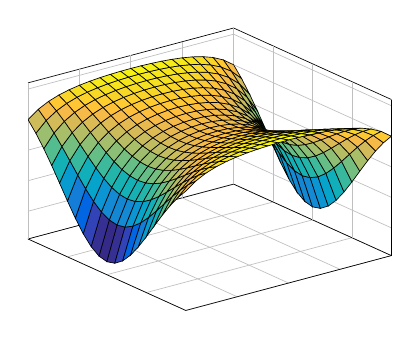
\begin{tikzpicture}[scale=0.6]

\begin{axis}[%
width=3.028in,
height=2.354in,
at={(1.011in,0.642in)},
scale only axis,
ticks=none,
%xmin=-1,
%xmax=1,
%tick align=outside,
xmajorgrids,
xtick = {-1,-0.5,0,0.5,1},
%ymin=-1,
%ymax=1,
ymajorgrids,
ytick = {-1,-0.5,0,0.5,1},
%zmin=-5,
%zmax=0,
zmajorgrids,
ztick = {-5,-4,-3,-2,-1,0,1},
view={-37.5}{30},
axis background/.style={fill=white}
%axis x line*=bottom,
%axis y line*=left,
%axis z line*=left
]

\addplot3[%
surf,
shader=flat corner,draw=black,z buffer=sort,colormap={mymap}{[1pt] rgb(0pt)=(0.2081,0.1663,0.5292); rgb(1pt)=(0.211624,0.189781,0.577676); rgb(2pt)=(0.212252,0.213771,0.626971); rgb(3pt)=(0.2081,0.2386,0.677086); rgb(4pt)=(0.195905,0.264457,0.7279); rgb(5pt)=(0.170729,0.291938,0.779248); rgb(6pt)=(0.125271,0.324243,0.830271); rgb(7pt)=(0.0591333,0.359833,0.868333); rgb(8pt)=(0.0116952,0.38751,0.881957); rgb(9pt)=(0.00595714,0.408614,0.882843); rgb(10pt)=(0.0165143,0.4266,0.878633); rgb(11pt)=(0.0328524,0.443043,0.871957); rgb(12pt)=(0.0498143,0.458571,0.864057); rgb(13pt)=(0.0629333,0.47369,0.855438); rgb(14pt)=(0.0722667,0.488667,0.8467); rgb(15pt)=(0.0779429,0.503986,0.838371); rgb(16pt)=(0.0793476,0.520024,0.831181); rgb(17pt)=(0.0749429,0.537543,0.826271); rgb(18pt)=(0.0640571,0.556986,0.823957); rgb(19pt)=(0.0487714,0.577224,0.822829); rgb(20pt)=(0.0343429,0.596581,0.819852); rgb(21pt)=(0.0265,0.6137,0.8135); rgb(22pt)=(0.0238905,0.628662,0.803762); rgb(23pt)=(0.0230905,0.641786,0.791267); rgb(24pt)=(0.0227714,0.653486,0.776757); rgb(25pt)=(0.0266619,0.664195,0.760719); rgb(26pt)=(0.0383714,0.674271,0.743552); rgb(27pt)=(0.0589714,0.683757,0.725386); rgb(28pt)=(0.0843,0.692833,0.706167); rgb(29pt)=(0.113295,0.7015,0.685857); rgb(30pt)=(0.145271,0.709757,0.664629); rgb(31pt)=(0.180133,0.717657,0.642433); rgb(32pt)=(0.217829,0.725043,0.619262); rgb(33pt)=(0.258643,0.731714,0.595429); rgb(34pt)=(0.302171,0.737605,0.571186); rgb(35pt)=(0.348167,0.742433,0.547267); rgb(36pt)=(0.395257,0.7459,0.524443); rgb(37pt)=(0.44201,0.748081,0.503314); rgb(38pt)=(0.487124,0.749062,0.483976); rgb(39pt)=(0.530029,0.749114,0.466114); rgb(40pt)=(0.570857,0.748519,0.44939); rgb(41pt)=(0.609852,0.747314,0.433686); rgb(42pt)=(0.6473,0.7456,0.4188); rgb(43pt)=(0.683419,0.743476,0.404433); rgb(44pt)=(0.71841,0.741133,0.390476); rgb(45pt)=(0.752486,0.7384,0.376814); rgb(46pt)=(0.785843,0.735567,0.363271); rgb(47pt)=(0.818505,0.732733,0.34979); rgb(48pt)=(0.850657,0.7299,0.336029); rgb(49pt)=(0.882433,0.727433,0.3217); rgb(50pt)=(0.913933,0.725786,0.306276); rgb(51pt)=(0.944957,0.726114,0.288643); rgb(52pt)=(0.973895,0.731395,0.266648); rgb(53pt)=(0.993771,0.745457,0.240348); rgb(54pt)=(0.999043,0.765314,0.216414); rgb(55pt)=(0.995533,0.786057,0.196652); rgb(56pt)=(0.988,0.8066,0.179367); rgb(57pt)=(0.978857,0.827143,0.163314); rgb(58pt)=(0.9697,0.848138,0.147452); rgb(59pt)=(0.962586,0.870514,0.1309); rgb(60pt)=(0.958871,0.8949,0.113243); rgb(61pt)=(0.959824,0.921833,0.0948381); rgb(62pt)=(0.9661,0.951443,0.0755333); rgb(63pt)=(0.9763,0.9831,0.0538)},mesh/rows=21]
table[row sep=crcr, point meta=\thisrow{c}] {%
%
x	y	z	c\\
-1	-1	-1	-1\\
-1	-0.9	-1.32976202812147	-1.32976202812147\\
-1	-0.8	-1.71600686218486	-1.71600686218486\\
-1	-0.7	-2.14899437465522	-2.14899437465522\\
-1	-0.6	-2.61169647342312	-2.61169647342312\\
-1	-0.5	-3.08021684891803	-3.08021684891803\\
-1	-0.4	-3.52542148736538	-3.52542148736538\\
-1	-0.3	-3.91572305199272	-3.91572305199272\\
-1	-0.2	-4.22069581699655	-4.22069581699655\\
-1	-0.1	-4.41496541277858	-4.41496541277858\\
-1	0	-4.48168907033806	-4.48168907033806\\
-1	0.1	-4.41496541277858	-4.41496541277858\\
-1	0.2	-4.22069581699655	-4.22069581699655\\
-1	0.3	-3.91572305199272	-3.91572305199272\\
-1	0.4	-3.52542148736538	-3.52542148736538\\
-1	0.5	-3.08021684891803	-3.08021684891803\\
-1	0.6	-2.61169647342312	-2.61169647342312\\
-1	0.7	-2.14899437465522	-2.14899437465522\\
-1	0.8	-1.71600686218486	-1.71600686218486\\
-1	0.9	-1.32976202812147	-1.32976202812147\\
-1	1	-1	-1\\
-0.9	-1	-0.752014254319383	-0.752014254319383\\
-0.9	-0.9	-1	-1\\
-0.9	-0.8	-1.29046162087289	-1.29046162087289\\
-0.9	-0.7	-1.61607440219289	-1.61607440219289\\
-0.9	-0.6	-1.96403297596985	-1.96403297596985\\
-0.9	-0.5	-2.31636697678109	-2.31636697678109\\
-0.9	-0.4	-2.65116721098261	-2.65116721098261\\
-0.9	-0.3	-2.94467955106552	-2.94467955106552\\
-0.9	-0.2	-3.1740234175276	-3.1740234175276\\
-0.9	-0.1	-3.32011692273655	-3.32011692273655\\
-0.9	0	-3.37029406432161	-3.37029406432161\\
-0.9	0.1	-3.32011692273655	-3.32011692273655\\
-0.9	0.2	-3.1740234175276	-3.1740234175276\\
-0.9	0.3	-2.94467955106552	-2.94467955106552\\
-0.9	0.4	-2.65116721098261	-2.65116721098261\\
-0.9	0.5	-2.31636697678109	-2.31636697678109\\
-0.9	0.6	-1.96403297596985	-1.96403297596985\\
-0.9	0.7	-1.61607440219289	-1.61607440219289\\
-0.9	0.8	-1.29046162087289	-1.29046162087289\\
-0.9	0.9	-1	-1\\
-0.9	1	-0.752014254319383	-0.752014254319383\\
-0.8	-1	-0.58274825237399	-0.58274825237399\\
-0.8	-0.9	-0.774916497961081	-0.774916497961081\\
-0.8	-0.8	-1	-1\\
-0.8	-0.7	-1.25232271619186	-1.25232271619186\\
-0.8	-0.6	-1.52196155561863	-1.52196155561863\\
-0.8	-0.5	-1.7949909856399	-1.7949909856399\\
-0.8	-0.4	-2.05443321064389	-2.05443321064389\\
-0.8	-0.3	-2.2818807653293	-2.2818807653293\\
-0.8	-0.2	-2.45960311115695	-2.45960311115695\\
-0.8	-0.1	-2.57281337858833	-2.57281337858833\\
-0.8	0	-2.61169647342312	-2.61169647342312\\
-0.8	0.1	-2.57281337858833	-2.57281337858833\\
-0.8	0.2	-2.45960311115695	-2.45960311115695\\
-0.8	0.3	-2.2818807653293	-2.2818807653293\\
-0.8	0.4	-2.05443321064389	-2.05443321064389\\
-0.8	0.5	-1.7949909856399	-1.7949909856399\\
-0.8	0.6	-1.52196155561863	-1.52196155561863\\
-0.8	0.7	-1.25232271619186	-1.25232271619186\\
-0.8	0.8	-1	-1\\
-0.8	0.9	-0.774916497961081	-0.774916497961081\\
-0.8	1	-0.58274825237399	-0.58274825237399\\
-0.7	-1	-0.465333930974313	-0.465333930974313\\
-0.7	-0.9	-0.618783391806141	-0.618783391806141\\
-0.7	-0.8	-0.798516218759377	-0.798516218759377\\
-0.7	-0.7	-1	-1\\
-0.7	-0.6	-1.21531098648973	-1.21531098648973\\
-0.7	-0.5	-1.43332941456034	-1.43332941456034\\
-0.7	-0.4	-1.64049823905704	-1.64049823905704\\
-0.7	-0.3	-1.82211880039051	-1.82211880039051\\
-0.7	-0.2	-1.96403297596985	-1.96403297596985\\
-0.7	-0.1	-2.05443321064389	-2.05443321064389\\
-0.7	0	-2.08548199250503	-2.08548199250503\\
-0.7	0.1	-2.05443321064389	-2.05443321064389\\
-0.7	0.2	-1.96403297596985	-1.96403297596985\\
-0.7	0.3	-1.82211880039051	-1.82211880039051\\
-0.7	0.4	-1.64049823905704	-1.64049823905704\\
-0.7	0.5	-1.43332941456034	-1.43332941456034\\
-0.7	0.6	-1.21531098648973	-1.21531098648973\\
-0.7	0.7	-1	-1\\
-0.7	0.8	-0.798516218759377	-0.798516218759377\\
-0.7	0.9	-0.618783391806141	-0.618783391806141\\
-0.7	1	-0.465333930974313	-0.465333930974313\\
-0.6	-1	-0.382892885975112	-0.382892885975112\\
-0.6	-0.9	-0.509156420607549	-0.509156420607549\\
-0.6	-0.8	-0.657046819815057	-0.657046819815057\\
-0.6	-0.7	-0.822834658056019	-0.822834658056019\\
-0.6	-0.6	-1	-1\\
-0.6	-0.5	-1.17939311871139	-1.17939311871139\\
-0.6	-0.4	-1.349858807576	-1.349858807576\\
-0.6	-0.3	-1.49930250005677	-1.49930250005677\\
-0.6	-0.2	-1.61607440219289	-1.61607440219289\\
-0.6	-0.1	-1.69045884837909	-1.69045884837909\\
-0.6	0	-1.71600686218486	-1.71600686218486\\
-0.6	0.1	-1.69045884837909	-1.69045884837909\\
-0.6	0.2	-1.61607440219289	-1.61607440219289\\
-0.6	0.3	-1.49930250005677	-1.49930250005677\\
-0.6	0.4	-1.349858807576	-1.349858807576\\
-0.6	0.5	-1.17939311871139	-1.17939311871139\\
-0.6	0.6	-1	-1\\
-0.6	0.7	-0.822834658056019	-0.822834658056019\\
-0.6	0.8	-0.657046819815057	-0.657046819815057\\
-0.6	0.9	-0.509156420607549	-0.509156420607549\\
-0.6	1	-0.382892885975112	-0.382892885975112\\
-0.5	-1	-0.32465246735835	-0.32465246735835\\
-0.5	-0.9	-0.43171052342908	-0.43171052342908\\
-0.5	-0.8	-0.557105861812174	-0.557105861812174\\
-0.5	-0.7	-0.697676326071031	-0.697676326071031\\
-0.5	-0.6	-0.847893704087916	-0.847893704087916\\
-0.5	-0.5	-1	-1\\
-0.5	-0.4	-1.14453678435131	-1.14453678435131\\
-0.5	-0.3	-1.2712491503214	-1.2712491503214\\
-0.5	-0.2	-1.370259310957	-1.370259310957\\
-0.5	-0.1	-1.43332941456034	-1.43332941456034\\
-0.5	0	-1.4549914146182	-1.4549914146182\\
-0.5	0.1	-1.43332941456034	-1.43332941456034\\
-0.5	0.2	-1.370259310957	-1.370259310957\\
-0.5	0.3	-1.2712491503214	-1.2712491503214\\
-0.5	0.4	-1.14453678435131	-1.14453678435131\\
-0.5	0.5	-1	-1\\
-0.5	0.6	-0.847893704087916	-0.847893704087916\\
-0.5	0.7	-0.697676326071031	-0.697676326071031\\
-0.5	0.8	-0.557105861812174	-0.557105861812174\\
-0.5	0.9	-0.43171052342908	-0.43171052342908\\
-0.5	1	-0.32465246735835	-0.32465246735835\\
-0.4	-1	-0.28365402649977	-0.28365402649977\\
-0.4	-0.9	-0.377192353563157	-0.377192353563157\\
-0.4	-0.8	-0.486752255959972	-0.486752255959972\\
-0.4	-0.7	-0.609570907296309	-0.609570907296309\\
-0.4	-0.6	-0.740818220681718	-0.740818220681718\\
-0.4	-0.5	-0.873715911688034	-0.873715911688034\\
-0.4	-0.4	-1	-1\\
-0.4	-0.3	-1.11071061035571	-1.11071061035571\\
-0.4	-0.2	-1.19721736312181	-1.19721736312181\\
-0.4	-0.1	-1.25232271619186	-1.25232271619186\\
-0.4	0	-1.2712491503214	-1.2712491503214\\
-0.4	0.1	-1.25232271619186	-1.25232271619186\\
-0.4	0.2	-1.19721736312181	-1.19721736312181\\
-0.4	0.3	-1.11071061035571	-1.11071061035571\\
-0.4	0.4	-1	-1\\
-0.4	0.5	-0.873715911688034	-0.873715911688034\\
-0.4	0.6	-0.740818220681718	-0.740818220681718\\
-0.4	0.7	-0.609570907296309	-0.609570907296309\\
-0.4	0.8	-0.486752255959972	-0.486752255959972\\
-0.4	0.9	-0.377192353563157	-0.377192353563157\\
-0.4	1	-0.28365402649977	-0.28365402649977\\
-0.3	-1	-0.255380675988078	-0.255380675988078\\
-0.3	-0.9	-0.339595525644939	-0.339595525644939\\
-0.3	-0.8	-0.438234992464949	-0.438234992464949\\
-0.3	-0.7	-0.548811636094027	-0.548811636094027\\
-0.3	-0.6	-0.666976810858474	-0.666976810858474\\
-0.3	-0.5	-0.786627861066553	-0.786627861066553\\
-0.3	-0.4	-0.900324522586266	-0.900324522586266\\
-0.3	-0.3	-1	-1\\
-0.3	-0.2	-1.07788415088463	-1.07788415088463\\
-0.3	-0.1	-1.12749685157938	-1.12749685157938\\
-0.3	0	-1.14453678435131	-1.14453678435131\\
-0.3	0.1	-1.12749685157938	-1.12749685157938\\
-0.3	0.2	-1.07788415088463	-1.07788415088463\\
-0.3	0.3	-1	-1\\
-0.3	0.4	-0.900324522586266	-0.900324522586266\\
-0.3	0.5	-0.786627861066553	-0.786627861066553\\
-0.3	0.6	-0.666976810858474	-0.666976810858474\\
-0.3	0.7	-0.548811636094027	-0.548811636094027\\
-0.3	0.8	-0.438234992464949	-0.438234992464949\\
-0.3	0.9	-0.339595525644939	-0.339595525644939\\
-0.3	1	-0.255380675988078	-0.255380675988078\\
-0.2	-1	-0.236927758682122	-0.236927758682122\\
-0.2	-0.9	-0.315057536903413	-0.315057536903413\\
-0.2	-0.8	-0.406569659740599	-0.406569659740599\\
-0.2	-0.7	-0.509156420607549	-0.509156420607549\\
-0.2	-0.6	-0.618783391806141	-0.618783391806141\\
-0.2	-0.5	-0.729788874269057	-0.729788874269057\\
-0.2	-0.4	-0.835270211411272	-0.835270211411272\\
-0.2	-0.3	-0.927743486328553	-0.927743486328553\\
-0.2	-0.2	-1	-1\\
-0.2	-0.1	-1.04602785990872	-1.04602785990872\\
-0.2	0	-1.06183654654536	-1.06183654654536\\
-0.2	0.1	-1.04602785990872	-1.04602785990872\\
-0.2	0.2	-1	-1\\
-0.2	0.3	-0.927743486328553	-0.927743486328553\\
-0.2	0.4	-0.835270211411272	-0.835270211411272\\
-0.2	0.5	-0.729788874269057	-0.729788874269057\\
-0.2	0.6	-0.618783391806141	-0.618783391806141\\
-0.2	0.7	-0.509156420607549	-0.509156420607549\\
-0.2	0.8	-0.406569659740599	-0.406569659740599\\
-0.2	0.9	-0.315057536903413	-0.315057536903413\\
-0.2	1	-0.236927758682122	-0.236927758682122\\
-0.1	-1	-0.226502340676469	-0.226502340676469\\
-0.1	-0.9	-0.301194211912202	-0.301194211912202\\
-0.1	-0.8	-0.388679570901753	-0.388679570901753\\
-0.1	-0.7	-0.486752255959972	-0.486752255959972\\
-0.1	-0.6	-0.591555364366815	-0.591555364366815\\
-0.1	-0.5	-0.697676326071031	-0.697676326071031\\
-0.1	-0.4	-0.798516218759377	-0.798516218759377\\
-0.1	-0.3	-0.886920436717158	-0.886920436717158\\
-0.1	-0.2	-0.9559974818331	-0.9559974818331\\
-0.1	-0.1	-1	-1\\
-0.1	0	-1.01511306461572	-1.01511306461572\\
-0.1	0.1	-1	-1\\
-0.1	0.2	-0.9559974818331	-0.9559974818331\\
-0.1	0.3	-0.886920436717158	-0.886920436717158\\
-0.1	0.4	-0.798516218759377	-0.798516218759377\\
-0.1	0.5	-0.697676326071031	-0.697676326071031\\
-0.1	0.6	-0.591555364366815	-0.591555364366815\\
-0.1	0.7	-0.486752255959972	-0.486752255959972\\
-0.1	0.8	-0.388679570901753	-0.388679570901753\\
-0.1	0.9	-0.301194211912202	-0.301194211912202\\
-0.1	1	-0.226502340676469	-0.226502340676469\\
0	-1	-0.22313016014843	-0.22313016014843\\
0	-0.9	-0.296710014294045	-0.296710014294045\\
0	-0.8	-0.382892885975112	-0.382892885975112\\
0	-0.7	-0.479505458974894	-0.479505458974894\\
0	-0.6	-0.58274825237399	-0.58274825237399\\
0	-0.5	-0.687289278790972	-0.687289278790972\\
0	-0.4	-0.786627861066553	-0.786627861066553\\
0	-0.3	-0.873715911688035	-0.873715911688035\\
0	-0.2	-0.941764533584249	-0.941764533584249\\
0	-0.1	-0.985111939603063	-0.985111939603063\\
0	0	-1	-1\\
0	0.1	-0.985111939603063	-0.985111939603063\\
0	0.2	-0.941764533584249	-0.941764533584249\\
0	0.3	-0.873715911688035	-0.873715911688035\\
0	0.4	-0.786627861066553	-0.786627861066553\\
0	0.5	-0.687289278790972	-0.687289278790972\\
0	0.6	-0.58274825237399	-0.58274825237399\\
0	0.7	-0.479505458974894	-0.479505458974894\\
0	0.8	-0.382892885975112	-0.382892885975112\\
0	0.9	-0.296710014294045	-0.296710014294045\\
0	1	-0.22313016014843	-0.22313016014843\\
0.1	-1	-0.226502340676469	-0.226502340676469\\
0.1	-0.9	-0.301194211912202	-0.301194211912202\\
0.1	-0.8	-0.388679570901753	-0.388679570901753\\
0.1	-0.7	-0.486752255959972	-0.486752255959972\\
0.1	-0.6	-0.591555364366815	-0.591555364366815\\
0.1	-0.5	-0.697676326071031	-0.697676326071031\\
0.1	-0.4	-0.798516218759377	-0.798516218759377\\
0.1	-0.3	-0.886920436717158	-0.886920436717158\\
0.1	-0.2	-0.9559974818331	-0.9559974818331\\
0.1	-0.1	-1	-1\\
0.1	0	-1.01511306461572	-1.01511306461572\\
0.1	0.1	-1	-1\\
0.1	0.2	-0.9559974818331	-0.9559974818331\\
0.1	0.3	-0.886920436717158	-0.886920436717158\\
0.1	0.4	-0.798516218759377	-0.798516218759377\\
0.1	0.5	-0.697676326071031	-0.697676326071031\\
0.1	0.6	-0.591555364366815	-0.591555364366815\\
0.1	0.7	-0.486752255959972	-0.486752255959972\\
0.1	0.8	-0.388679570901753	-0.388679570901753\\
0.1	0.9	-0.301194211912202	-0.301194211912202\\
0.1	1	-0.226502340676469	-0.226502340676469\\
0.2	-1	-0.236927758682122	-0.236927758682122\\
0.2	-0.9	-0.315057536903413	-0.315057536903413\\
0.2	-0.8	-0.406569659740599	-0.406569659740599\\
0.2	-0.7	-0.509156420607549	-0.509156420607549\\
0.2	-0.6	-0.618783391806141	-0.618783391806141\\
0.2	-0.5	-0.729788874269057	-0.729788874269057\\
0.2	-0.4	-0.835270211411272	-0.835270211411272\\
0.2	-0.3	-0.927743486328553	-0.927743486328553\\
0.2	-0.2	-1	-1\\
0.2	-0.1	-1.04602785990872	-1.04602785990872\\
0.2	0	-1.06183654654536	-1.06183654654536\\
0.2	0.1	-1.04602785990872	-1.04602785990872\\
0.2	0.2	-1	-1\\
0.2	0.3	-0.927743486328553	-0.927743486328553\\
0.2	0.4	-0.835270211411272	-0.835270211411272\\
0.2	0.5	-0.729788874269057	-0.729788874269057\\
0.2	0.6	-0.618783391806141	-0.618783391806141\\
0.2	0.7	-0.509156420607549	-0.509156420607549\\
0.2	0.8	-0.406569659740599	-0.406569659740599\\
0.2	0.9	-0.315057536903413	-0.315057536903413\\
0.2	1	-0.236927758682122	-0.236927758682122\\
0.3	-1	-0.255380675988078	-0.255380675988078\\
0.3	-0.9	-0.339595525644939	-0.339595525644939\\
0.3	-0.8	-0.438234992464949	-0.438234992464949\\
0.3	-0.7	-0.548811636094027	-0.548811636094027\\
0.3	-0.6	-0.666976810858474	-0.666976810858474\\
0.3	-0.5	-0.786627861066553	-0.786627861066553\\
0.3	-0.4	-0.900324522586266	-0.900324522586266\\
0.3	-0.3	-1	-1\\
0.3	-0.2	-1.07788415088463	-1.07788415088463\\
0.3	-0.1	-1.12749685157938	-1.12749685157938\\
0.3	0	-1.14453678435131	-1.14453678435131\\
0.3	0.1	-1.12749685157938	-1.12749685157938\\
0.3	0.2	-1.07788415088463	-1.07788415088463\\
0.3	0.3	-1	-1\\
0.3	0.4	-0.900324522586266	-0.900324522586266\\
0.3	0.5	-0.786627861066553	-0.786627861066553\\
0.3	0.6	-0.666976810858474	-0.666976810858474\\
0.3	0.7	-0.548811636094027	-0.548811636094027\\
0.3	0.8	-0.438234992464949	-0.438234992464949\\
0.3	0.9	-0.339595525644939	-0.339595525644939\\
0.3	1	-0.255380675988078	-0.255380675988078\\
0.4	-1	-0.28365402649977	-0.28365402649977\\
0.4	-0.9	-0.377192353563157	-0.377192353563157\\
0.4	-0.8	-0.486752255959972	-0.486752255959972\\
0.4	-0.7	-0.609570907296309	-0.609570907296309\\
0.4	-0.6	-0.740818220681718	-0.740818220681718\\
0.4	-0.5	-0.873715911688034	-0.873715911688034\\
0.4	-0.4	-1	-1\\
0.4	-0.3	-1.11071061035571	-1.11071061035571\\
0.4	-0.2	-1.19721736312181	-1.19721736312181\\
0.4	-0.1	-1.25232271619186	-1.25232271619186\\
0.4	0	-1.2712491503214	-1.2712491503214\\
0.4	0.1	-1.25232271619186	-1.25232271619186\\
0.4	0.2	-1.19721736312181	-1.19721736312181\\
0.4	0.3	-1.11071061035571	-1.11071061035571\\
0.4	0.4	-1	-1\\
0.4	0.5	-0.873715911688034	-0.873715911688034\\
0.4	0.6	-0.740818220681718	-0.740818220681718\\
0.4	0.7	-0.609570907296309	-0.609570907296309\\
0.4	0.8	-0.486752255959972	-0.486752255959972\\
0.4	0.9	-0.377192353563157	-0.377192353563157\\
0.4	1	-0.28365402649977	-0.28365402649977\\
0.5	-1	-0.32465246735835	-0.32465246735835\\
0.5	-0.9	-0.43171052342908	-0.43171052342908\\
0.5	-0.8	-0.557105861812174	-0.557105861812174\\
0.5	-0.7	-0.697676326071031	-0.697676326071031\\
0.5	-0.6	-0.847893704087916	-0.847893704087916\\
0.5	-0.5	-1	-1\\
0.5	-0.4	-1.14453678435131	-1.14453678435131\\
0.5	-0.3	-1.2712491503214	-1.2712491503214\\
0.5	-0.2	-1.370259310957	-1.370259310957\\
0.5	-0.1	-1.43332941456034	-1.43332941456034\\
0.5	0	-1.4549914146182	-1.4549914146182\\
0.5	0.1	-1.43332941456034	-1.43332941456034\\
0.5	0.2	-1.370259310957	-1.370259310957\\
0.5	0.3	-1.2712491503214	-1.2712491503214\\
0.5	0.4	-1.14453678435131	-1.14453678435131\\
0.5	0.5	-1	-1\\
0.5	0.6	-0.847893704087916	-0.847893704087916\\
0.5	0.7	-0.697676326071031	-0.697676326071031\\
0.5	0.8	-0.557105861812174	-0.557105861812174\\
0.5	0.9	-0.43171052342908	-0.43171052342908\\
0.5	1	-0.32465246735835	-0.32465246735835\\
0.6	-1	-0.382892885975112	-0.382892885975112\\
0.6	-0.9	-0.509156420607549	-0.509156420607549\\
0.6	-0.8	-0.657046819815057	-0.657046819815057\\
0.6	-0.7	-0.822834658056019	-0.822834658056019\\
0.6	-0.6	-1	-1\\
0.6	-0.5	-1.17939311871139	-1.17939311871139\\
0.6	-0.4	-1.349858807576	-1.349858807576\\
0.6	-0.3	-1.49930250005677	-1.49930250005677\\
0.6	-0.2	-1.61607440219289	-1.61607440219289\\
0.6	-0.1	-1.69045884837909	-1.69045884837909\\
0.6	0	-1.71600686218486	-1.71600686218486\\
0.6	0.1	-1.69045884837909	-1.69045884837909\\
0.6	0.2	-1.61607440219289	-1.61607440219289\\
0.6	0.3	-1.49930250005677	-1.49930250005677\\
0.6	0.4	-1.349858807576	-1.349858807576\\
0.6	0.5	-1.17939311871139	-1.17939311871139\\
0.6	0.6	-1	-1\\
0.6	0.7	-0.822834658056019	-0.822834658056019\\
0.6	0.8	-0.657046819815057	-0.657046819815057\\
0.6	0.9	-0.509156420607549	-0.509156420607549\\
0.6	1	-0.382892885975112	-0.382892885975112\\
0.7	-1	-0.465333930974313	-0.465333930974313\\
0.7	-0.9	-0.618783391806141	-0.618783391806141\\
0.7	-0.8	-0.798516218759377	-0.798516218759377\\
0.7	-0.7	-1	-1\\
0.7	-0.6	-1.21531098648973	-1.21531098648973\\
0.7	-0.5	-1.43332941456034	-1.43332941456034\\
0.7	-0.4	-1.64049823905704	-1.64049823905704\\
0.7	-0.3	-1.82211880039051	-1.82211880039051\\
0.7	-0.2	-1.96403297596985	-1.96403297596985\\
0.7	-0.1	-2.05443321064389	-2.05443321064389\\
0.7	0	-2.08548199250503	-2.08548199250503\\
0.7	0.1	-2.05443321064389	-2.05443321064389\\
0.7	0.2	-1.96403297596985	-1.96403297596985\\
0.7	0.3	-1.82211880039051	-1.82211880039051\\
0.7	0.4	-1.64049823905704	-1.64049823905704\\
0.7	0.5	-1.43332941456034	-1.43332941456034\\
0.7	0.6	-1.21531098648973	-1.21531098648973\\
0.7	0.7	-1	-1\\
0.7	0.8	-0.798516218759377	-0.798516218759377\\
0.7	0.9	-0.618783391806141	-0.618783391806141\\
0.7	1	-0.465333930974313	-0.465333930974313\\
0.8	-1	-0.58274825237399	-0.58274825237399\\
0.8	-0.9	-0.774916497961081	-0.774916497961081\\
0.8	-0.8	-1	-1\\
0.8	-0.7	-1.25232271619186	-1.25232271619186\\
0.8	-0.6	-1.52196155561863	-1.52196155561863\\
0.8	-0.5	-1.7949909856399	-1.7949909856399\\
0.8	-0.4	-2.05443321064389	-2.05443321064389\\
0.8	-0.3	-2.2818807653293	-2.2818807653293\\
0.8	-0.2	-2.45960311115695	-2.45960311115695\\
0.8	-0.1	-2.57281337858833	-2.57281337858833\\
0.8	0	-2.61169647342312	-2.61169647342312\\
0.8	0.1	-2.57281337858833	-2.57281337858833\\
0.8	0.2	-2.45960311115695	-2.45960311115695\\
0.8	0.3	-2.2818807653293	-2.2818807653293\\
0.8	0.4	-2.05443321064389	-2.05443321064389\\
0.8	0.5	-1.7949909856399	-1.7949909856399\\
0.8	0.6	-1.52196155561863	-1.52196155561863\\
0.8	0.7	-1.25232271619186	-1.25232271619186\\
0.8	0.8	-1	-1\\
0.8	0.9	-0.774916497961081	-0.774916497961081\\
0.8	1	-0.58274825237399	-0.58274825237399\\
0.9	-1	-0.752014254319383	-0.752014254319383\\
0.9	-0.9	-1	-1\\
0.9	-0.8	-1.29046162087289	-1.29046162087289\\
0.9	-0.7	-1.61607440219289	-1.61607440219289\\
0.9	-0.6	-1.96403297596985	-1.96403297596985\\
0.9	-0.5	-2.31636697678109	-2.31636697678109\\
0.9	-0.4	-2.65116721098261	-2.65116721098261\\
0.9	-0.3	-2.94467955106552	-2.94467955106552\\
0.9	-0.2	-3.1740234175276	-3.1740234175276\\
0.9	-0.1	-3.32011692273655	-3.32011692273655\\
0.9	0	-3.37029406432161	-3.37029406432161\\
0.9	0.1	-3.32011692273655	-3.32011692273655\\
0.9	0.2	-3.1740234175276	-3.1740234175276\\
0.9	0.3	-2.94467955106552	-2.94467955106552\\
0.9	0.4	-2.65116721098261	-2.65116721098261\\
0.9	0.5	-2.31636697678109	-2.31636697678109\\
0.9	0.6	-1.96403297596985	-1.96403297596985\\
0.9	0.7	-1.61607440219289	-1.61607440219289\\
0.9	0.8	-1.29046162087289	-1.29046162087289\\
0.9	0.9	-1	-1\\
0.9	1	-0.752014254319383	-0.752014254319383\\
1	-1	-1	-1\\
1	-0.9	-1.32976202812147	-1.32976202812147\\
1	-0.8	-1.71600686218486	-1.71600686218486\\
1	-0.7	-2.14899437465522	-2.14899437465522\\
1	-0.6	-2.61169647342312	-2.61169647342312\\
1	-0.5	-3.08021684891803	-3.08021684891803\\
1	-0.4	-3.52542148736538	-3.52542148736538\\
1	-0.3	-3.91572305199272	-3.91572305199272\\
1	-0.2	-4.22069581699655	-4.22069581699655\\
1	-0.1	-4.41496541277858	-4.41496541277858\\
1	0	-4.48168907033806	-4.48168907033806\\
1	0.1	-4.41496541277858	-4.41496541277858\\
1	0.2	-4.22069581699655	-4.22069581699655\\
1	0.3	-3.91572305199272	-3.91572305199272\\
1	0.4	-3.52542148736538	-3.52542148736538\\
1	0.5	-3.08021684891803	-3.08021684891803\\
1	0.6	-2.61169647342312	-2.61169647342312\\
1	0.7	-2.14899437465522	-2.14899437465522\\
1	0.8	-1.71600686218486	-1.71600686218486\\
1	0.9	-1.32976202812147	-1.32976202812147\\
1	1	-1	-1\\
};
\end{axis}
\end{tikzpicture}% 
    \caption{Quadratic non-convex surface.}
    \label{nonconvexfig}
  \end{minipage}
  \label{fig:nonlinearpumps}
\end{figure}
%The gradient of the objective function tells the direction in which the change has the greatest rate. In case of convexity, this gradient vector points in the direction of the global minimum, therefore using iterative methods it can be found easily.

 \figref{convexfig} and \figref{nonconvexfig} points out the differences between the two minimization problems. Solving the convex quadratic problem will results in obtaining the global minimum, which can be found determining the first derivative of the function and solving it for to zero. 
 In order to ensure convexity, the objective function must have a positive semi-definite Hessian matrix. The Hessian is a square matrix of second order partial derivatives of a scalar-valued function or scalar field. Therefore, to obtain an expression that fulfills this condition, the Hessian for \eqref{eq:obj_final1} is analyzed : 

\begin{align}
%
\Upsilon(\bm{\hat{u}}_{\bm{Hp}}) &= \frac{1}{\eta}\bigg( \frac{1}{2} \bm{\hat{u}}_{\bm{Hp}}^{T} \bm{R} \bm{\hat{u}}_{\bm{Hp}} + \bm{b} \bm{\hat{u}}_{\bm{Hp}} + c \bigg)\\
%
\frac{\partial \Upsilon(\bm{\hat{u}}_{\bm{Hp}})}{\partial \bm{\hat{u}}_{\bm{Hp}}} &= \frac{1}{\eta}\cdot \big(\bm{R} \bm{\hat{u}}_{\bm{Hp}} + \bm{b} \big)\\
%
\frac{\partial^2 \Upsilon(\bm{\hat{u}}_{\bm{Hp}})}{\partial {\bm{\hat{u}}}^{2}_{\bm{Hp}}} &= \frac{1}{\eta}\cdot \bm{R} 
\label{hessian}
%
\end{align}

\eqref{hessian} shows that convexity is ensured if:

\begin{equation}
\bm{R} \succeq 0  
\end{equation}

for all $\bm{\hat{u}}_{\bm{Hp}} $, since the efficiency, $\eta$ is a positive constant, therefore does not change the convexity of the function. 

Recalling \eqref{R_quadratic}, $\bm{R}$ depends on $\bm{\Lambda_1}$ from \eqref{pumpflows_simplified}, which is defined as $\bm{\Lambda_1} =\bm{G^T} \bm{B_{1}^T}\bm{M_c^{-1}}\bm{N_c}$.

Bringing back the structure of $N_c = B_1$, the above equation can be rewritten as:

\begin{equation}
\bm{\Lambda_1} =\bm{N_c}^{T} \bm{M_c^{-1}}\bm{N_c}
\end{equation}

In \secref{} $\bm{M_c}$ has been defined as a symmetric positive definite matrix, the same procedure as in \eqref{PosDefi} is followed. The above equation is multiplied by a non-zero vector column $\bm{x}$ and its transpose $\bm{x}^{T}$

\begin{equation}
	\bm{x}^{T}\bm{N_c}^{T} \bm{M_c^{-1}}\bm{N_c}\bm{x}
\end{equation}

A new variable is defined $\bm{y} = \bm{N_c}\bm{x}$, now making usage of the definition of positive definiteness 

\begin{equation}
	\bm{y}^{T} \bm{M_c^{-1}} \bm{y} \geqslant 0
	\label{Def_Mc}
\end{equation}

 With $\bm{M_c}$ fulfilling the requirements for positive definiteness, the Hessian $\bm{R}$ can be certified to be greater than zero, hence convex.
 % Every term in this expression is known and positive semi-definite, except $\bm{M_c}$, which includes all the resistance terms as an outcome of the parameter estimation. Therefore $\bm{M_c}$ must be positive semi-definite. To ensure that the objective function is convex, this requirement has been explained in detail in the formulation of \eqref{statespace_control_sys_state}.  

% The definition of a convex function can be written as, $\triangledown(\triangledown g(\cdot)) \geq 0$,  and the definition of a strictly convex function as $\triangledown(\triangledown g(\cdot)) > 0$. For the purpose of this project is it only required for the optimization problem to be convex. 





%
%\begin{align}
%\underset{\bm{\hat{u}_{Hp}}}{min} \:  \Upsilon(\cdot) &= \underset{\bm{\hat{u}_{Hp}}}{min} \:  \frac{1}{\eta}\bigg( \frac{1}{2} \bm{\hat{u}}_{\bm{Hp}}^{T} \bm{R} \bm{\hat{u}}_{\bm{Hp}} + \bm{b} \bm{\hat{u}}_{\bm{Hp}} + c \bigg)\\
%
%\Upsilon(\cdot) &= \frac{1}{\eta}\bigg( \frac{1}{2} \bm{\hat{u}}_{\bm{Hp}}^{T} \bm{R} \bm{\hat{u}}_{\bm{Hp}} + \bm{b} \bm{\hat{u}}_{\bm{Hp}} + c \bigg)\\
%
%\triangledown \Upsilon(\cdot) &= \frac{1}{\eta}\cdot \big(\bm{R} \bm{\hat{u}}_{\bm{Hp}} + \bm{b} \big)\\
%
%\triangledown(\triangledown \Upsilon(\cdot)) &= \frac{1}{\eta}\cdot \bm{R} 
%
%\end{align}



\textbf{Constraints}

The constraints are given by linear inequalities which define half-spaces that are contained the quadratic function. A half-space is half-space is a set of points that satisfy a single inequality constraint, hence, each constraint defines a half-space \cite{van2005formulation}. Every half-space is a convex set and the intersection of any number of convex sets is convex \cite{Convex_constraints}.
% The convexity of the constraints is investigated with the same procedure as for the objective function. All constraints are linear and the Hessian of a linear function, $Ax+b$, is always zero. Therefore the constraints are always convex.

%In this section:
%\\
%-show how the quadratic problem can be solved
%-prove positive semi-definiteness
